\documentclass{article}
\usepackage[utf8]{inputenc}
\usepackage{minted}
\usepackage{newunicodechar}
\usepackage[a4paper, margin=3cm]{geometry}
\usepackage{verbatim}
\usepackage{graphicx}

\newunicodechar{⏷}{\textdownarrow}
\newunicodechar{⏵}{\textrightarrow}

\title{Laporan Tugas Struktur Data}
\author{Muhammad Haekal Muhyidin Al-Araby \\ 5024221030}
\date{}

\begin{document}
\maketitle

\section{Source Code}
\subsection{Interpreter}
\inputminted{python3}{D:/PyProj/interpreted-lang-py/interpreter.py}
\subsection{Text Editor}
\inputminted{python3}{D:/PyProj/interpreted-lang-py/App.py}
\subsection{Logic Operation}
\inputminted{python3}{D:/PyProj/interpreted-lang-py/LogicOperation.py}
\subsection{Syntax Identifier}
\inputminted{python3}{D:/PyProj/interpreted-lang-py/syntax_identifier.py}
\section{Alur Program}
\subsection{Interpreter}
Interpreter adalah program console yang akan membaca suatu perintah lalu menjalankan perintah tersebut. 
Terdapat dua mode yaitu interactive mode dan non-interactive mode. Non-interactive mode dapat dijalankan 
dengan command py interpreter.py [namafile]. Sedangkan interactive mode dapat dijalankan dengan 
command py interpreter.py atau py interpreter.py -i [namafile]. Non-interactive akan membaca dan mengeksekusi
file lalu selesai. Sedangkan interactive akan membaca dan mengeksekusi file bila diberikan lalu membaca input 
dari user. Bila diberikan input file maka interpreter akan membaca file tersebut lalu mengeksekusi string yang didapat
dengan fungsi execstring dari class Interpreter. Pada fungsi execstring, string akan dipecah menjadi per baris. Lalu
diiterasikan dan diperiksa apakah string atau bagian dari string itu adalah block atau tidak. Bila tidak maka akan 
langsung dimasukkan pada fungsi \texttt{execline}. Bila iya maka akan memanggil fungsi \texttt{exec\_if}, \texttt{exec\_while}, 
\texttt{def\_fn}, \texttt{def\_class} tergantung dari jenis block tersebut. 
\subsubsection{Fungsi \texttt{execline}}
Fungsi execline akan menghapus seluruh line yang ada di belakang ''\#''. Selanjutnya akan diperiksa apakah ada goto atau tidak. Jika iya maka fungsi \texttt{exec\_goto} akan
dijalankan. Dimana fungsi tersebut akan menjalankan lagi command pada label yang dituju.
Selanjutnya diperiksa import. Dimana akan dijalankan \texttt{exec\_file} untuk file pada import.
Selanjutnya akan masuk \texttt{check\_assignment} dimana pada fungsi akan dicari index dari tanda ''=''. Bila tidak ada maka 
akan di jalankan fungsi \texttt{check\_keyword}. Bila ada maka akan dipisah menjadi dua bagian yaitu variabel dan value. Lalu akan dijalankan \texttt{check\_operation} untuk value.
dan dimasukkan ke dalam variabel. Yang dimana variabel tersebut bisa berupa variable biasa, array, atau variabel pada class. Bila variabel tidak ditemukan
maka akan dibuat variabel baru dan diappend pada list variabel pada interpreter. Bila ditemukan maka akan diubah nilainya.
\subsubsection{Fungsi \texttt{check\_operation}}
Pada \texttt{check\_operation} akan diperiksa apakah array atau tidak. Bila
iya maka akan mereturn array yang dimana tiap elemennya akan dijalankan \texttt{check\_operation} lagi. 
Bila tidak maka akan akan dibagi tiap elemennya dengan operator arithmetic maupun logic. Sebelumnya
tiap string pada input akan disembunyikan agar tidak terpisah. Setelah semua operasi
untuk memecah strin akan didapat list yang terdiri dari Operator dan Operand. dimana
operand sendiri akan diperiksa kembali apakah memanggil fungsi atau tidak. variable atau bukan.
yang dimana akan cari nilai dari operand tersebut. Bila berhasil maka list tersebut
akan dihitung menggunakan diolah menjadi postfix lalu dihitung. Bila gagal akan dikembalikan elemen pertama atau None
\subsubsection{Fungsi \texttt{check\_keyword}}
Pada fungsi ini akan diperiksa apakah fungsi tersebut adalah built-in function, fungsi atau class yang sudah define. Yang akan menjalankan 
fungsi yang tersimpan lalu mengembalikan hasilnya. Bila tidak maka akan mengembalikan None.
\subsubsection{Fungsi \texttt{exec\_if}}
Fungsi ini akan mengambil kondisi dan block code dibawahnya lalu dimasukkan list kondisi dan list task yang akan dijalankan. Dimana kondisi akan 
diperiksa nilainya dengan fungsi \texttt{check\_operation} bila nilainya 1 maka block code dibawahnya dijalankan dengan fungsi \texttt{exec\_string}
bila tidak maka akan memeriksa
kondisi setelahnya. Dan seterusnya dimana untuk else diberikan nilai 1 langsung.
\subsubsection{Fungsi \texttt{exec\_while}}
Fungsi ini akan menggunakan while loop dimana kondisi yang diberikan adalah nilai return \\ \texttt{check\_operation}. Dimana dimana pada while dijalankan
fungsi \texttt{exec\_string} untuk block code yang ada di dalam while.
\subsubsection{Fungsi \texttt{def\_fn}}
Fungsi ini akan menyimpan nama fungsi, argumen, dan block code yang akan dijalankan. Dimana bila fungsi dipanggil maka
akan dibuat interpreter baru sebagai scope variabel lalu argument akan dimasukkan pada sebagai variabel pada interpreter baru
tersebut. 
\subsubsection{Fungsi \texttt{def\_class}}
Fungsi ini akan menyimpan nama class, argumen, fungsi pada class. Dimana saat class akan diinstantiate akan
dibuat interpreter baru untuk scope class tersebut. Dimana seluruh block code pada class akan dijalankan untuk memasukkan
fungsi dan variable pada class tersebut. Selanjuta fungsi pada class dapat dipanggil dengan menggunakan \texttt{nama\_class.nama\_fungsi}
pada fungsi dalam class untuk mereferensi class tersebut dapat menggunakan \texttt{this}. Class adalah mutable object
sehingga bila dimasukkan pada fungsi, elemen pada class dapat dirubah.
\subsection{Text Editor}
Text Editor dapat membuka folder atau file. Lalu ditampilkan pada Aplikasi. Program ini menggunakan
library customtkinter dan beberapa dari tkinter untuk tampilannya. Program ini mampu syntax highlighting
untuk bahasa pemrograman yang saya buat dimana data didapat dari syntax identifier. Lalu program dapat menjalankan code pada textbox.
dengan menggunakan subprocess untuk menjalankan program interpreter. Program ini juga dilengkapi dengan interactive terminal
dimana cara kerja dari interactive terminal adalah menjalankan subprocess untuk menjalankan program interpreter. 
Lalu terdapat input yang dapat tiap kali ditekan enter maka isinya akan dikirim ke proc.stdin Lalu dijalankan
oleh interpreter. Lalu output dari interpreter akan ditampilkan pada terminal. Untuk menampilkan output dari terminal
saya menggunakan thread baru agar tidak mengganggu main thread. Dimana thread tersebut akan menjalankan fungsi \texttt{read\_proc} lalu 
dioutputkan pada textbox yang dibuat seolah olah seperti terminal. 
\subsection{Syntax Identifier}
Syntax Identifier adalah program yang akan mengidentifikasi syntax dari suatu file. Program ini akan membaca file lalu mendeteksi setiap keyword yang sudah
ditentukan ia juga dapat mendeteksi variable, fungsi, dan class yang dibuat user. hasilnya akan dibaca text editor untuk 
syntax highlighting.
\section{Contoh Input \& Output}
\subsection{Input}
\subsubsection{\texttt{code\_example.pyhk}}
\verbatiminput{D:/PyProj/interpreted-lang-py/code_example.pyhk}
\subsubsection{\texttt{Lib/vector\_class.pyhk}}
\verbatiminput{D:/PyProj/interpreted-lang-py/Lib/vector_class.pyhk}
\subsection{Output}
\verbatiminput{D:/PyProj/interpreted-lang-py/output.txt}
\subsection{Screenshot}
\begin{figure}[H]
    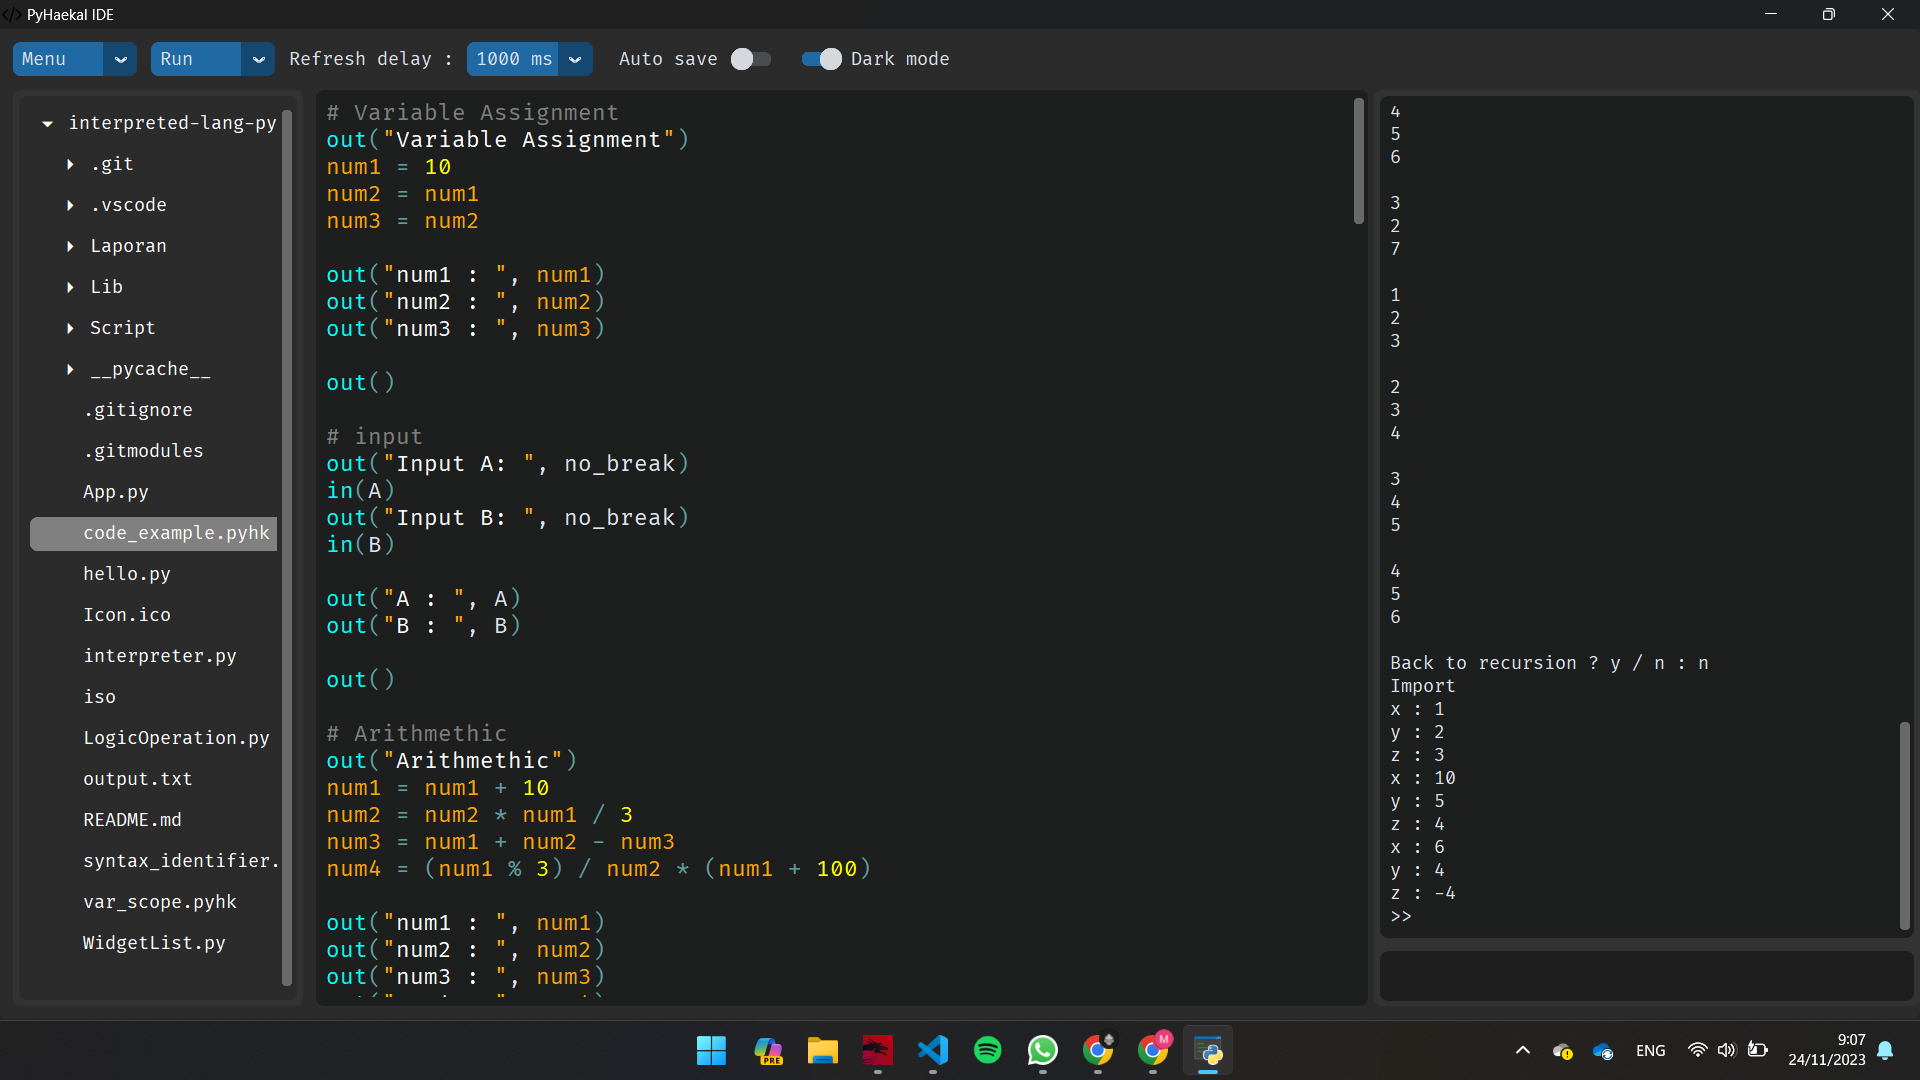
\includegraphics[width=\textwidth]{image1.png}
    \caption{Screenshot Text Editor}
\end{figure}
\end{document}